	%\documentclass[english]{sareport}
% use the option peerreview for creating an anonymized version of your report
% E.g., \documentclass[english,peerreview]{sareport}

\usepackage[colorlinks, linkcolor=black, citecolor=black, urlcolor=black]{hyperref}
\usepackage{float}


% Set all authors, if your group counts 2, set third author empty \authorthree{}
% Set the groupname as well
\authorone{Robin Haveneers (r0450702)}
\authortwo{Stef Verreydt (r0456110)}
\authorthree{Axel Lemmens (r0462440)}
\groupname{Haveneers-Verreydt-Lemmens}

\academicyear{2016--2017}

\casename{Shared Internet Of Things Infrastructure Platform}
\phasenumber{1}
\phasename{Domain Analysis}


\begin{document}
\maketitle

\tableofcontents

\chapter{Domain analysis}\label{sec:domain}
\section{Domain models}
This sections contains the domain models for our system. For readability reasons, the model is split into two parts. In the first figure the general domain model is shown, in the second figure the model containing the hardware and information flow is illustrated.

\begin{figure}[H]
    \centering
    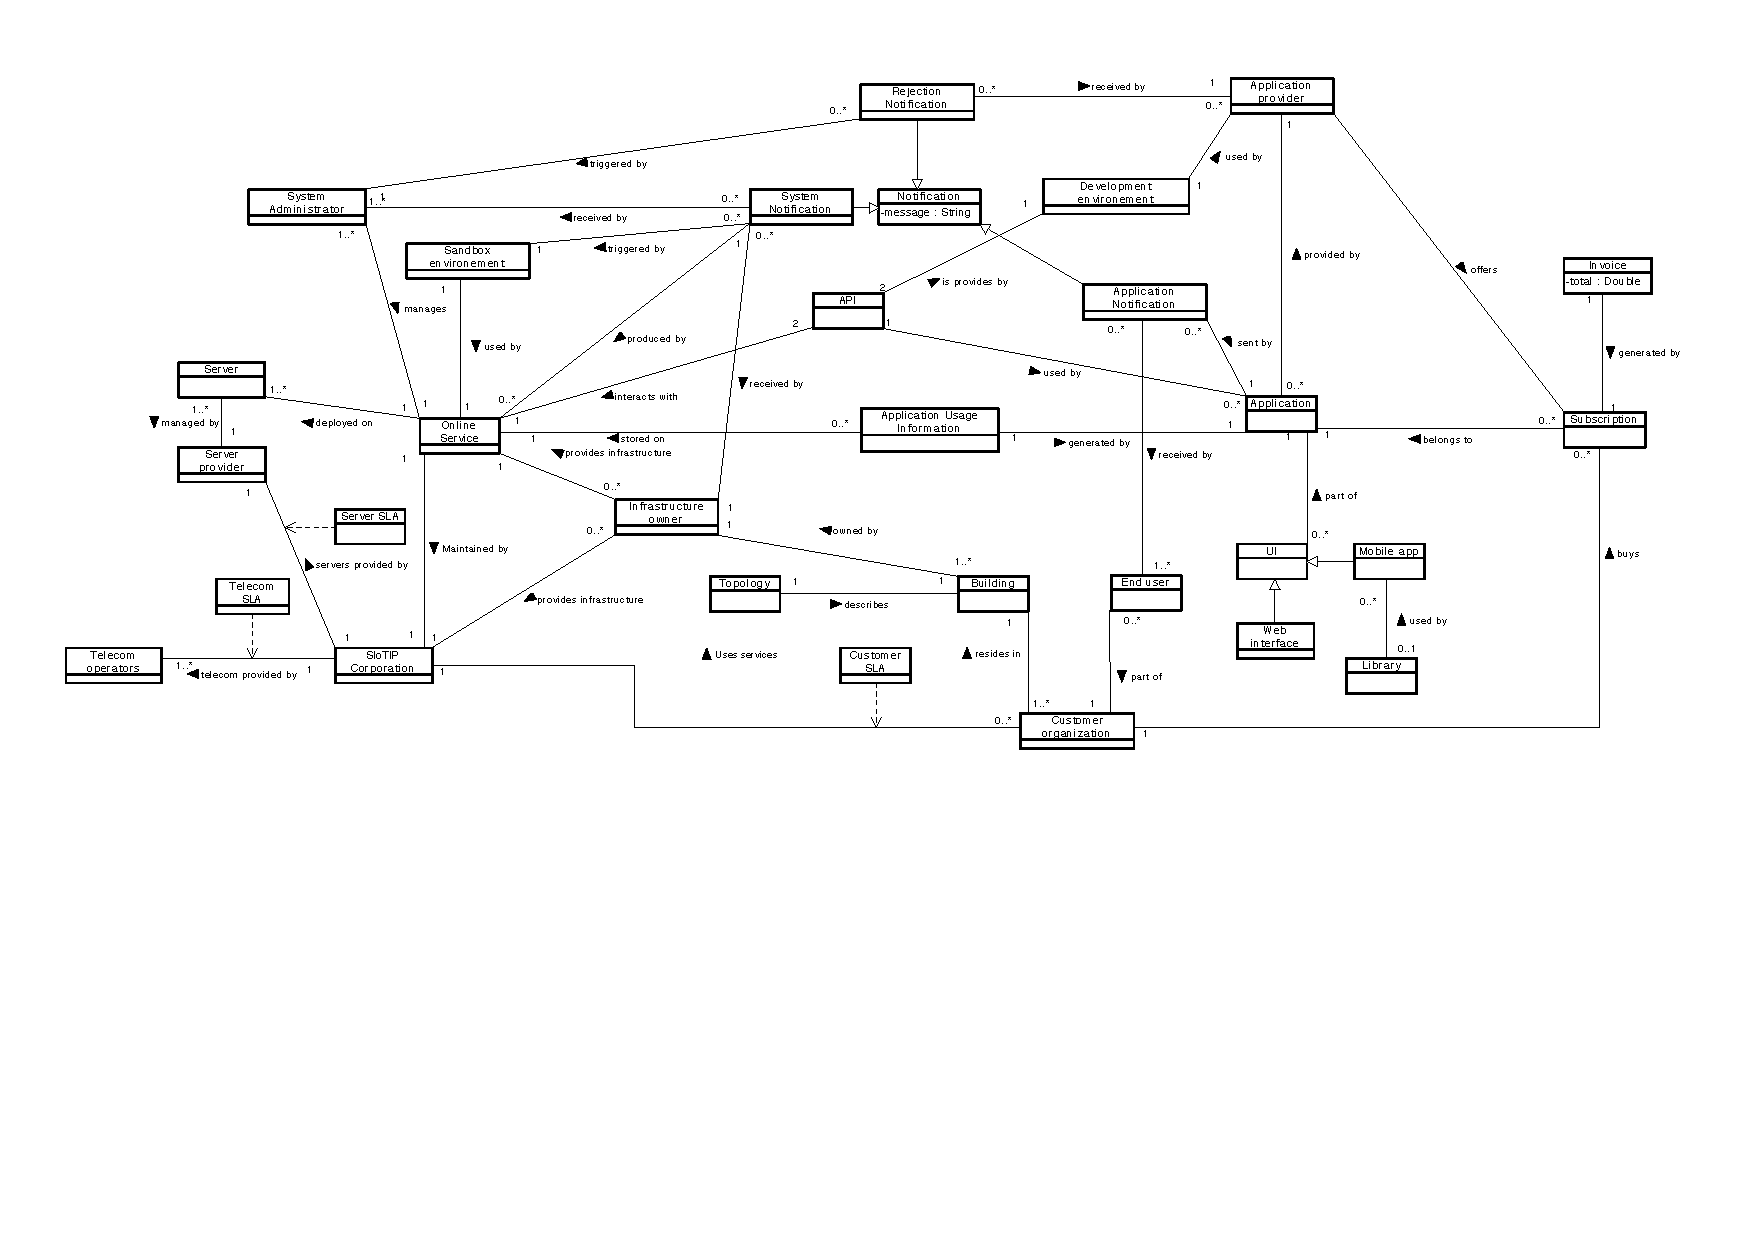
\includegraphics[width=\textwidth, height=9cm, angle=90]{Domain_model.pdf}
    \caption{Domain model: General}\label{fig:domain_model1}
\end{figure}

\begin{figure}[H]
    \centering
    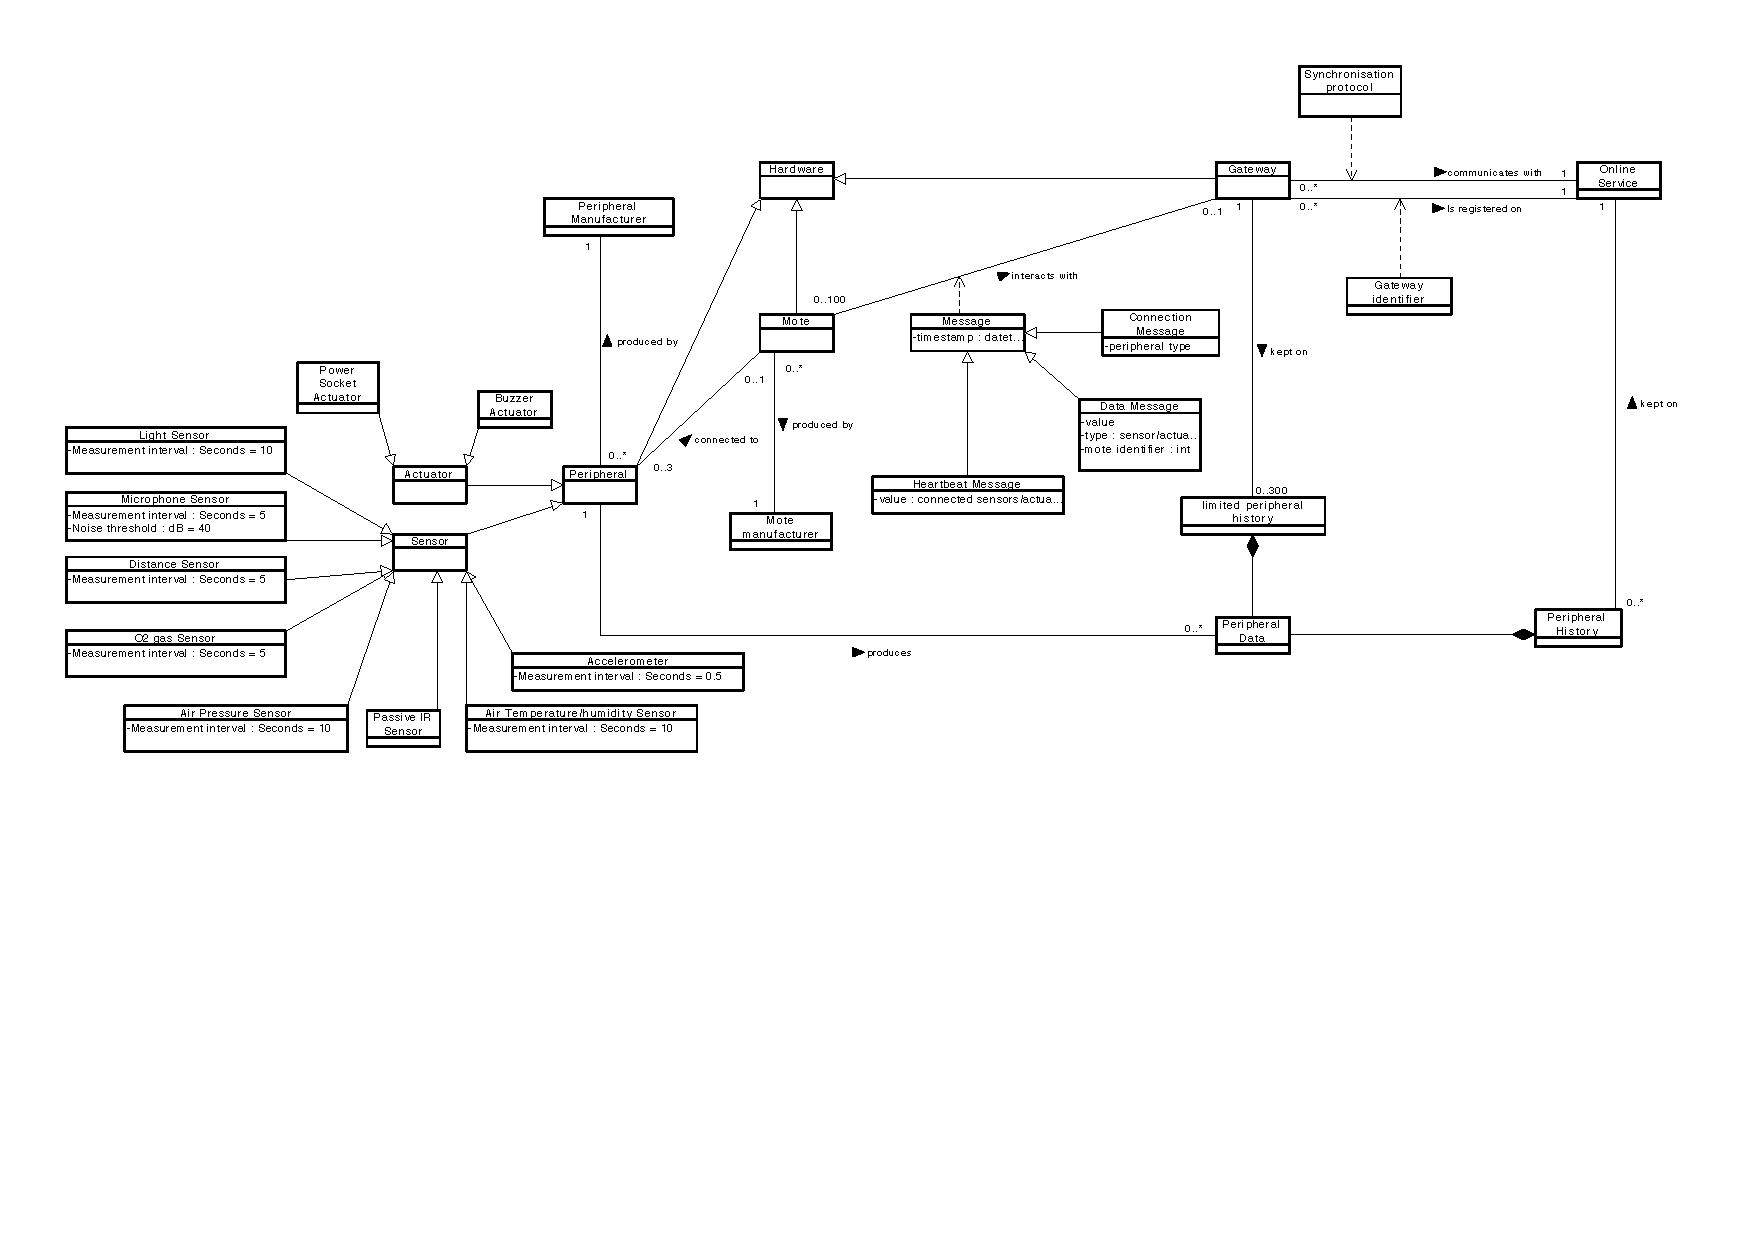
\includegraphics[width=\textwidth, height=9cm, angle=90]{Hardware_and_information_flow.pdf}
    \caption{Domain model: Hardware and information flow}\label{fig:domain_model2}
\end{figure}

\section{Domain constraints}
In this section we provide additional domain constraints.

\begin{itemize}
    \item A customer organisation can only subscribe to an application that is already registered with the system.
    \item A end-user only receives notifications from applications that the customer organisation he works for is subscribed to. He only receives these notifications if he/she is an individual who should receive notifications as configured in the application by the previously mentioned customer organisation.
    \item The Online Service can only communicate with peripherals via their gateway.
    \item The connectivity between the network manager and the attached devices is done via 6LoWPAN.
    \item Application developers only receive rejection notifications about the applications they want to deploy.
    \item An application should be idle until all the necessary hardware is available and if the hardware is available it should be activated automatically. For example, a fire application requires at least 2 specific sensors per room.
    \item If a component of the hardware fails, the system should automatically switch to a nearby, similar device if possible, based on the topology provided by the infrastructure owner.
    \item Only persons who are allowed to do so, can issue commands to an application.
    \item Gateways contain limited storage space. Whenever they're running low on space, the oldest information should be removed.
    \item When communicating with the system, customer organisations, infrastructure owners, system administrators and application providers each have their own, personal, dashboard to do so.
\end{itemize}

\section{Glossary}
In this section, we provide a glossary of the most important terminology used
in this analysis.

\begin{itemize}
	\item \textbf{API}: Application programming interface. The interface used by applications to communicate with the online system and gateways.
	\item \textbf{Accelerometer}: Type of sensor that measures the acceleration in 3 dimensions.
	\item \textbf{Actuator}: Hardware device that has actions associated with it (e.g. switch, light, buzzer ...)
	\item \textbf{Air Pressure Sensor}: Type of sensor that measures the air pressure in bar.
	\item \textbf{Air Temperature/Humidity Sensor}: Type of sensor the measures the air temperature in degrees Celsius and humidity in percentage.
	\item \textbf{Application Notification}: A type of notification send by the application to a relevant end-user.
	\item \textbf{Application Usage Information}: Data collected by applications and stored on the online service. Useful for providing insight in application usage and big data analytics.
	\item \textbf{Application provider}: Stakeholder that provides (develops and deploys) applications on the online system, to which one can subscribe.
	\item \textbf{Application}: Piece of 'software' running on the online service and gateway provided to customer organisations to subscribe to with the goal of simplifying their day to day business.
	\item \textbf{Building}: Place owned by infrastructure owner where customer organisations are housed. The infrastructure owners keeps a topology about the building they own.
	\item \textbf{Buzzer}: Actuator that is able to play a sound.
	\item \textbf{Connection Message}: The message that is sent by the mote to the gateway whenever a new sensor or actuator is inserted.
	\item \textbf{Customer SLA}: The Service-Level Agreement between SIoTIP corporation and the customer organisation.
	\item \textbf{Customer organisation}: The stakeholder in our system which subscribes to applications which optimise their workflow.
	\item \textbf{Data Message}: The message send by the mote from one of its connected devices to the gateway which contains the value it's reading, the mote identifier and a timestamp. This message also specifies whether it was sent by a sensor/actuator which is necessary to be able to correctly interpret the data.
	\item \textbf{Development environment}: The environment available to application providers to freely test and debug their application before deploying it.
	\item \textbf{Distance Sensor}: Type of sensor which measure 
	\item \textbf{End user}: A person involved in the customer organisation who interacts with applications.
	\item \textbf{Gateway identifier}: The identifier which is used to register the gateway with the Online Service.
	\item \textbf{Gateway}: A device that is connected to the online service and which provides access to sensors and actuators. It relays data from connected devices to the Online Service.
	\item \textbf{Hardware}: Umbrella concept used for all the connected devices (such as peripherals, gateways ...)
	\item \textbf{Heartbeat Message}: Periodical message sent by the mote to indicate it is alive. This message includes a list of connected sensors and actuators as well as a timestamp indicating when the message was generated.
	\item \textbf{Infrastructure owner}: Stakeholder in our system which manages the physical infrastructure as well as the hardware used as described in the topology. Customer organisations reside in these buildings.
	\item \textbf{Invoice}: An invoice is associated with a subscription between a customer organisation and an application provider. It specifies the fees necessary to be paid by the customer organisation.
	\item \textbf{Light Sensor}: Type of sensor that measures the amount of light in LUX.
	\item \textbf{Message}: Umbrella term used for the different types of messages a mote can emit.
	\item \textbf{Microphone Sensor}: Type of sensor which allows detection of sound. 
	\item \textbf{Mobile app}: One type of interface end-users can use to communicate with the online system.
	\item \textbf{Mote manufacturer}: Third party which produces the motes used by our system.
	\item \textbf{Mote}: Device that hosts sensors and actuators.
	\item \textbf{Notification}: Umbrella concept used for all the different types of notifications used by the system. Notifications are sent out on several events. The precise information depends on the type of event.
	\item \textbf{O$_2$ gas sensor}: Sensor that can measure the amount of O$_2$ gas in the air  in percentage.
	\item \textbf{Online Service}: The collective concept that are the services provided via our online back-end. This service is used to test, develop and host applications, to store application configurations, keep track of sensor data, collect usage statistics etc. 
	\item \textbf{Passive IR (Presence) Sensor}: Type of sensor which allows detection of motion achieved by taking pictures and comparing subsequent pictures.
	\item \textbf{Peripheral Data}: The data which is produced by peripherals/hardware.
	\item \textbf{Peripheral Manufacturer}: The third party company that is responsible for the manufacturing of sensors and actuators.
	\item \textbf{Peripheral Type}: The type of the peripheral. Currently sensor and actuator are possible.
	\item \textbf{Peripheral}: Umbrella concept for sensors and actuators.
	\item \textbf{Power socket}: Type of actuator which can be turned on or off.
	\item \textbf{Rejection Notification}: The type of notification which is triggered by the sandbox environment if the application that is waiting to be deployed is rejected by our system. This notification is send to the application provider.
	\item \textbf{SIoTIP Corporation}: This stakeholder wants SIoTIP to be a successful platform for deploying IoT devices. They have agreements with different third parties for providing an optimal platform with respect to availability, performance ..
	\item \textbf{Sandbox environment}: The environment which is used to test submitted applications before they become available on the Online Service. When there are problems with the application being tested, a system administrator performs a secondary, manual review. If he rejects the application, the application provider is notified and is required to fix the application.
	\item \textbf{Sensor}: A type of peripheral that produces measurements and sends this data to the gateway to be used in applications.
	\item \textbf{Server provider}: The third-party provider which provides (virtual or physical) servers to deploy the Online Service on.
	\item \textbf{Server}: The server (virtual or physical) on which the Online Service is deployed. They are provided by the third party server provider.
	\item \textbf{Server SLA}: The SLA between SIoTIP corporation and the server provider which, among others, specifies the up-time constraints and reaction time in case of a hardware failure.
	\item \textbf{Subscription}: An agreement between the application provider and a customer organisation in which is specified for which application a customer organisation is subscribed.
	\item \textbf{Synchronisation protocol}: The protocol used in the communication between the gateways and the online service.
	\item \textbf{System Administrator}: The person responsible to act when a submitted application is rejected. He or she can accept the application nonetheless or reject it as well which notifies the application provider.
	\item \textbf{System Notification}: A notification which notifies the system administrator when a submitted application needs attention. This notification is triggered by the sandbox environment.
	\item \textbf{Telecom SLA}: The SLA between the SIoTIP corporation and the telecom provider which specifies the the capabilities of these communication channels.
	\item \textbf{Telecom operators}: Third party who provides means for gateways to communicate with the Online Service and vice versa.
	\item \textbf{Topology}: Overview of the hardware of the infrastructure spread out over the building(s) he owns. This can be used when new, for example, new applications are added to find out which new hardware is necessary.
	\item \textbf{UI}: The interface of a application used by end users of a customer organisation.
	\item \textbf{Web interface}: A possible UI for an application used by end users to communicate with the online service.
\end{itemize}

\chapter{Functional requirements}\label{sec:functional}
\section*{Use case model}

\begin{figure}[H]
    \centering
    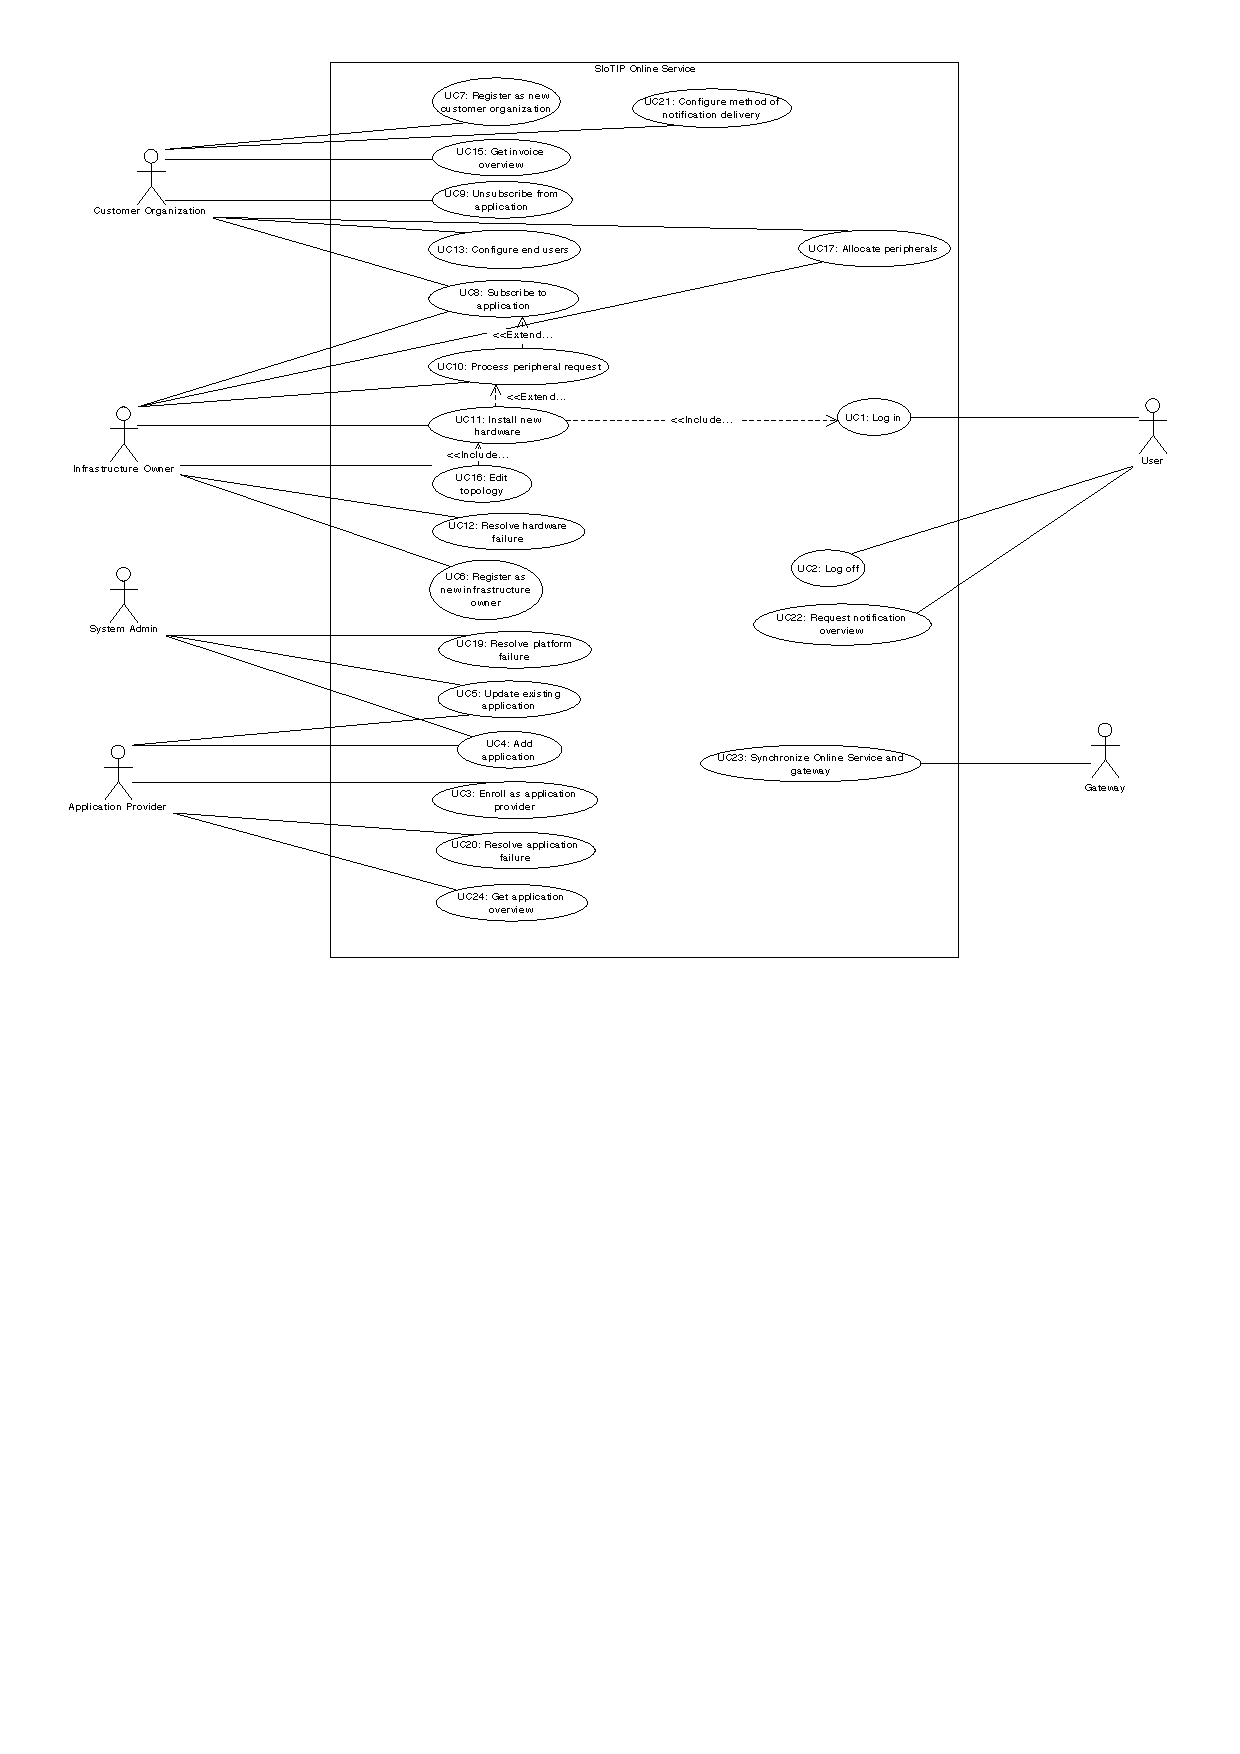
\includegraphics[width=\textwidth]{Use_Case_Diagram.pdf}
    \caption{Use case diagram} (main functional requirements) \label{fig:Use_Case_Diagram}
\end{figure}

\section{Use case overview}\label{sec:uc_overview}
\paragraph{UC1: Log in}
The user wishing to use the system provides his credentials.
The Online Service verifies the credentials and authenticates the user.
The Online Service then provides the user access to his dashboard.
If the provides credentials were not correct, the system does not authenticate the user.

\paragraph{UC2: Log out}
The user indicates he wants to log off from the system.
The system logs him of.

\paragraph{UC3: Enroll as application provider}
The organisation wishing to become a an Application Provider contacts SIoTIP and they negotiate the contract. The organisation receives API documentation and rules of conduct from SIoTIP. When the negotiations are conducted, the organisation is provided dashboard accounts for the individual developers employed by the organisation and the organisation is registered as an Application Provider in the Online service.

\paragraph{UC4: Add application}
The user logs into the his Application Provider dashboard and uploads the new application. The Online Service initiates a number of automated tests and shows the progress on the user's Application Provider dashboard. If the application passes all tests, the user receives a notification and the application is made available to Customer organisations for subscription. If the application does not pass al tests, a SIoTIP System Administrator performs a secondary review and decides whether to accept or reject the application. In the latter case, the user is notified of the reason of rejection.

\paragraph{UC5: Update existing application}
The user logs into the his Application Provider dashboard and uploads the updated application. The user also indicates whether to automatically update existing instances of the application or to require customer organisations to subscribe to the application. The Online Service initiates a number of automated tests and shows the progress on the user's application provider dashboard. If the application passes all tests, the user receives a notification and the application is made available to customer organisations for subscription. If the application does not pass all tests, a SIoTIP system administrator performs a secondary review and decides whether to accept or reject the application. In the latter case, the user is notified of the reason of rejection.

\paragraph{UC6: Register as new infrastructure owner}
The infrastructure owner contacts SIoTIP and negotiations are started. An Infrastructure Owner dashboard account is set up for the new user. The infrastructure owner provides the names of the currently renting companies, and SIoTIP contacts them for registration (See UC: Register new customer organisation).

\paragraph{UC7: Register as new customer organisation}
The organisation contacts or is contacted by SIoTIP and provides it's billing and contact information. The organisation is then registered as a Customer organisation in the Online Service.

\paragraph{UC8: Subscribe to application}
The user logs into his Customer organisation dashboard, subscribes to the application and provides the needed information. The user is informed by the Online Service that the application will be activated once the required peripherals are installed. The Online Service checks whether or not the customer organisation has access to all the peripherals needed for the application. If not, the infrastructure owner is automatically notified of the subscription and the peripherals and gateways needed for that application (see UC10: process hardware request). Once all required hardware is installed, the application is activated and the user is notified.

\paragraph{UC9: Unsubscribe from application}
The user logs into his Customer organisation dashboard and unsubscribes from the application. The user is informed by the Online Service that the application will be deactivated.

\paragraph{UC10: Process hardware request}
The Infrastructure Owner is notified of a new request for hardware. The infrastructure owner approves or rejects the purchase of the hardware and a notification of the decision is sent to the customer organisation which requested the peripherals. If the infrastructure owner approves the request, the hardware is ordered from SIoTIP.

\paragraph{UC11: Install new hardware}
The Infrastructure Owner receives the hardware from SIoTIP and installs it. The infrastructure owner configures any new gateways to connect to the local network. Once online, the gateways immediately connect to the Online Service to register themselves. The infrastructure owner then logs in to the infrastructure owner dashboard and provides the necessary topology information. Lastly, he allocates the new peripherals to the Customer organisations in his building (See UC: Allocate peripherals).

\paragraph{UC12: Resolve hardware failure}
The Online Service detects that a hardware component is no longer sending data and sends a notification to the Infrastructure Owner. The Online Service also notifies all applications currently using the failing hardware component so that the applications can search for equivalent sensors in the topology. 

\paragraph{UC13: Configure end-users}
The user logs in to his Customer organisation dashboard and assigns users to an application. These changes are saved in the Online Service.

\paragraph{UC14: Transmit data}
The sensor sends data to the corresponding gateway. The gateway stores the data and makes it available to all applications interacting with the sensor.

\paragraph{UC15: Get invoice overview}
The user logs into his Customer organisation dashboard and selects the option to show his Customer organisation's invoice overview. The Online Service then shows an overview of all the Customer organisation's invoices.

\paragraph{UC16: Edit topology}
The user logs into his Infrastructure Owner dashboard and selects the option to edit the topology of his buildings. When the user is done editing the topology, the updated topology will be saved in the Online Service.

\paragraph{UC17: Allocate peripherals}
The user logs into his Infrastructure Owner dashboard and selects the option to allocate peripherals to Customer organisations. He then assigns access rights to the Customer organisations in his building to use the new peripherals. The Online Service automatically activates any application of that Customer Organisation which needed the newly allocated peripherals in order to run. Conversely, if a peripheral gets withheld from a Customer organisation, the Online Service deactivates any application of that Customer organisation which needed the witheld peripheral to function properly.

\paragraph{UC18: Resolve platform failure}
An event causes the platform to misbehave. The Online Service detects this event and sends a notification to the System Administrator(s).

\paragraph{UC19: Resolve application failure}
An event causes an application to misbehave. The Online Service detects this event and sends a notification to the System Administrator(s and a log is sent to the relevant Application Provider.

\paragraph{UC20: Configure method of notification delivery}
The user logs into his Customer organisation dashboard and configures the method of notification delivery. The Online Service will save the changes made.

\paragraph{UC21: Request notification overview}
The user logs into his dashboard and requests an overview of previously received notifications and alarms. The Online Service provides this overview.

\paragraph{UC22: Synchronize Online Service and gateway}
The gateway sends all data acquired between this moment and the last synchronisation moment to the Online Service.

\paragraph{UC23: Get application overview}
The user logs into his Application Provider dashboard and request an overview their applications. The Online Service provides this overview.


\section{Detailed use cases}

\subsection{\emph{UC4}: Add application}
\begin{itemize}
    \item \textbf{Name:} Add application
    \item \textbf{Primary actor:} Application Provider
    \item \textbf{Secondary actor(s)}: System Administrator, Online Service
    \item \textbf{Interested parties:} 
        \begin{itemize}
            \item \textit{Online Service:} wants to authenticate its users and keep track of applications.
            \item \textit{Application Provider:} wants his applications to be available on the SIoTIP platform.
        \end{itemize}

    \item \textbf{Preconditions:}
        \begin{itemize}
            \item The Application Provider is registered on the Online Service (cf. UC3).
            \item The Application Provider is logged into the Online Service (cf. UC1).
        \end{itemize}

    \item \textbf{Postconditions:}
        \begin{itemize}
            \item The Application Provider is notified about whether or not the application got accepted by the Online Service
        \end{itemize}
        
    \item \textbf{Main scenario:} 
    \begin{enumerate}
       \item The Application Provider indicates he wants to add an application
       \item The Online Service presents the Application Provider with a means to add his application to the Online Service.
       \item The Application Provider adds the application.
	\item The Online Service initiates a number of automated tests on the application.
	\item The application passes all tests.
	\item The Online Service notifies the Application Provider that the application got accepted.
       \item \ldots
    \end{enumerate}

    \item \textbf{Alternative scenarios:} 
    \begin{enumerate}
        \item [5b.] The application did not pass all automated tests.
	\begin{enumerate}
		\item [5b1.] The Online Service instructs a System Administrator to perform a secondary review.
		\item [5b2a.] The System administrator approves the application, resume at step 6.
		\item [5b2b.] The System Administrator rejects the application. The Application provider is notified of this decision.
	\end{enumerate}
    \end{enumerate}
\end{itemize}

\subsection{\emph{UC8}: Subscribe to application}
\begin{itemize}
    \item \textbf{Name:} Subscribe to application
    \item \textbf{Primary actor:} Customer organisation
    \item \textbf{Secondary actor(s)}: Infrastructure owner, Online Service
    \item \textbf{Interested parties:} 
        \begin{itemize}
            \item \textit{Online Service:} wants to authenticate its users and keep track of subscriptions.
            \item \textit{Customer organisation:} wants to subscribe to applications
            \item \textit{Infrastructure Owner:} Has to decide whether hardware will be bought for the applications or not.
        \end{itemize}

    \item \textbf{Preconditions:}
        \begin{itemize}
            \item The Customer organisation is registered on the Online Service (UC7).
            \item The member of the Customer organisation is logged into hit Customer organisation dashboard (cf. UC1).
        \end{itemize}

    \item \textbf{Postconditions:}
        \begin{itemize}
            \item The Customer organisation is subscribed to the application.

        \end{itemize}

        
    \item \textbf{Main scenario:} 
    \begin{enumerate}
       \item The member of the Customer organisation indicates he wants to subscribe to an application.
       \item The Online Service presents the user with a means to search for and subscribe to applications.
       \item The user subscribes to an application.
	\item The Online Service saves the subscription.
	\item The Online Service notifies the user that the application will be activated once the required peripherals are installed.
	\item The Online Service notifies the Infrastructure Owner that new peripherals are needed (\textbf{Include:} UC10: Process peripheral request).
	\item The Infrastructure Owner installs the hardware (\textbf{Include:} UC11: Install new hardware).
    \item The Infrastructure Owner allocates the new peripherals to the Customer organisation (\textbf{Include:} UC17: Allocate peripherals )
	\item The Online Service activates the application
	\item The Online Service notifies the user that the application is activated.
    \end{enumerate}

    \item \textbf{Alternative scenarios:} 
    \begin{enumerate}
        \item [3b.] Alternative at step 3
    \end{enumerate}
\end{itemize}


\subsection{\emph{UC10}: Process hardware request}
\begin{itemize}
    \item \textbf{Name:} Process peripheral request
    \item \textbf{Primary actor:} Infrastructure Owner
    \item \textbf{Secondary actor(s)}: Online Service
    \item \textbf{Interested parties:} 
        \begin{itemize}
            \item \textit{Customer organisations:} Could use the requested hardware if it is allocated to them.
            \item \textit{Infrastructure Owner:} Has to decide whether or not the hardware will be bought.
        \end{itemize}

    \item \textbf{Preconditions:}
        \begin{itemize}
            \item The Infrastructure Owner received a request for new hardware.
            \item The Infrastructure Owner is registered on the Online Service (cf. UC6).
            \item The Infrastructure Owner is logged into his Infrastructure Owner dashboard. (cf. UC1)
        \end{itemize}

    \item \textbf{Postconditions:}
        \begin{itemize}
            \item The requester of the hardware is notified about whether or not the Infrastructure Owner approved the request.
        \end{itemize}
        
    \item \textbf{Main scenario:} 
    \begin{enumerate}
       \item The Infrastructure Owner approves the request.
       \item The Online Service orders the hardware from SIoTIP.
       \item The Online Service notifies the requester of the hardware about the decision.
    \end{enumerate}

    \item \textbf{Alternative scenarios:} 
    \begin{enumerate}
        \item [1b1.] The Infrastructure Owner rejects the request, resume at step 3.
    \end{enumerate}
\end{itemize}

\subsection{\emph{UC11}: Install new hardware}
\begin{itemize}
    \item \textbf{Name:} Install new hardware
    \item \textbf{Primary actor:} Infrastructure Owner
    \item \textbf{Secondary actor(s)}: 
    \item \textbf{Interested parties:} 
        \begin{itemize}
            \item \textit{Online Service:}  wants to authenticate its users and keep track of all hardware.
            \item \textit{Customer organisations:} can use the newly installed hardware if it is allocated to them.
            \item \textit{Infrastructure Owner:} has to maintain topology of the hardware and has to place and configure it.
        \end{itemize}

    \item \textbf{Preconditions:}
        \begin{itemize}
            \item The Infrastructure Owner is registered on the Online Service (cf. UC6).
        \end{itemize}

    \item \textbf{Postconditions:}
        \begin{itemize}
            \item The new hardware is installed.
            \item The new hardware is added to the topology of the building it is installed in.
        \end{itemize}
        
    \item \textbf{Main scenario:} 
    \begin{enumerate}
       \item The Infrastructure Owner receives the hardware from SIoTIP.
       \item The Infrastructure Owner places the new hardware where it needs to be.
       \item The Infrastructure Owner configures any new gateways to connect to the local network.
       \item The new gateways automatically connect to the Online Service and register themselves.
       \item The Infrastructure Owner logs into the Online Service. (\textbf{Include:} UC1: log in)
       \item The Infrastructure Owner edits the topology of his infrastructure. (\textbf{Include:} UC16: Edit topology)
       \item The Infrastructure Owner allocates the new peripherals to the Customer organisations who are allowed to use them. (\textbf{UC17: Allocate peripherals})
    \end{enumerate}
\end{itemize}


\subsection{\emph{UC17}: Allocate peripherals}
\begin{itemize}
    \item \textbf{Name:} Allocate peripherals
    \item \textbf{Primary actor:} Infrastructure Owner
    \item \textbf{Secondary actor(s)}: Online Service
    \item \textbf{Interested parties:} 
        \begin{itemize}
             \item \textit{Online Service:}  wants to authenticate its users and keep track of all allocations.
             \item \textit{Customer organisations: } can use the peripherals if they are allocated to them.
        \end{itemize}

    \item \textbf{Preconditions:}
        \begin{itemize}
            \item The Infrastructure Owner is registered on the Online Service (cf. UC6).
            \item The Infrastructure Owner is logged into his Infrastructure Owner dashboard. (cf. UC1)
        \end{itemize}

    \item \textbf{Postconditions:}
        \begin{itemize}
            \item
        \end{itemize}

        
    \item \textbf{Main scenario:} 
    \begin{enumerate}
       \item The Infrastructure Owner indicates he wants to allocate or withhold peripherals to/from Customer organisations.
       \item The Online Service presents the user with a means to do this.
       \item The Infrastructure Owner allocates/withholds peripherals to/from Customer organisations.
       \item The Online Service activates any application in a Customer organisation which needed the peripherals allocated to that Customer organisation.
       \item The Online Service deactivates any application in a Customer organisation which needed the peripherals withheld from that Customer organisation.
    \end{enumerate}
\end{itemize}

\chapter{Non-functional requirements}\label{sec:non-functional}
In this section, we model the non-functional requirements for the system in the
form of \emph{quality attribute scenarios}. We provide for each type
(availability, performance and modifiability) one requirement.

\section{Availability}
\subsection{\emph{Av1}: Communication channel between the gateway and the Online Service}
Due to a failure of the intermediate telecom infrastructure or an error in/outage of the Online Service important functionalities of the Online Service are compromised: applications can not connect to the connected sensors/actuators to push modifications or get data.
\begin{itemize}
    \item \textbf{Source:} external or internal (e.g. error in the Online Service which results in a loss of connection between gateway and Online Service).
    \item \textbf{Stimulus:}
        \begin{itemize}
            \item the external communication channel between the gateway and the online service is failing
            \item or, the internal communication service of the Online Service is failing and thus connection between applications and gateways is not possible
        \end{itemize}

    \item \textbf{Artifact:} external communication channel, gateway, internal communication system
    \item \textbf{Environment:} normal execution
    \item \textbf{Response:}
        \begin{itemize}
            \item Prevention:
            \begin{itemize}
            	\item the SIoTIP corporation has negotiated a SLA with the telecom provider which stipulates 97\% availability over our communication channel 
            	\item the SIoTIP corporation has negotiated a SLA with the server provider which provides 99\% uptime of the servers used to run our Online Service
            	\item the gateways itself run minimal applications to ensure that when the connection to the Online Service is lost the actuators can still be used (e.g. temperature control)
            \end{itemize}
            \item Detection:
            \begin{itemize}
            	\item the gateways are able to detect that the Online Service is offline by receiving time-outs when sending data to the Online Service (e.g. when the external communication channel fails)
            	\item the Online Service detects the lack of updates from gateways and keeps track of how long no updates have been received
            \end{itemize}
            \item Resolution:\\
            In every scenario the system administrator is contacted.
            \begin{itemize}
            	\item if the external communication channel is at fault, the system administrator must contact the telecom provider to have this resolved
            	\item if the internal communication fails the system administrator resolves the technical issue and communication is automatically restored
            \end{itemize}
        \end{itemize}

    \item \textbf{Response measure:}
        \begin{itemize}
            \item Detection of a failing external or internal communication link depends on the synchronisation protocol but happens within one minute.
            \item In case of an external communication failure, the SLA with the telecom provider stipulates that the problem is addressed within 15 minutes and resolved within one hour. 
            \item In case of an internal communication failure, the system administrator has to resolve the issue within 20 minutes.
        \end{itemize}
\end{itemize}

\subsection{\emph{Av2}: Availability of microPnP sensors}
Due to the failure of a sensor, the correct behaviour of a critical application is compromised.
\begin{itemize}
    \item \textbf{Source:} external
    \item \textbf{Stimulus:}
        \begin{itemize}
            \item A sensor that is in use by a critical application (e.g. a fire alarm application) stopped working due to unforeseen circumstances (e.g. faulty battery in mote).
        \end{itemize}

    \item \textbf{Artifact:} the application
    \item \textbf{Environment:} normal execution
    \item \textbf{Response:}
        \begin{itemize}
            \item Prevention:
            \begin{itemize}
            	\item the system administrator has to check the battery level on all motes periodically.
            	\item the mote manufacturer guarantees a battery life of at least 3 years.
            	\item the sensor manufacturer guarantees a lifetime of at least 5 years.
            \end{itemize}
            \item Detection:
            \begin{itemize}
            	\item The online service detects the lack of incoming data.
            \end{itemize}
            \item Resolution:\\
            In every scenario the system administrator is contacted and the broken sensor is replaced.
            \begin{itemize}
            	\item If a alternative sensor can be found to replace the failing sensor, this sensor is used as a substitute.
            	\item if no alternative sensor can be found, the application and the infrastructure owner are notified.
            \end{itemize}
        \end{itemize}

    \item \textbf{Response measure:}
        \begin{itemize}
            \item the detection of a sensor failure happens within 30 seconds.
            \item in case of the presence of an alternative sensor the replacement in the application should be within 30 seconds.
        \end{itemize}
\end{itemize}
\section{Performance}
\subsection{\emph{P1}: Transferring data from sensor to Online Service}
Transferring periodic data from the sensors to the applications should happen in a timely fashion, even if a lot of sensors send at the same time.

\begin{itemize}
    \item \textbf{Source:} Sensor data
    \item \textbf{Stimulus:}
        \begin{itemize}
            \item synchronisation of data with the online service
        \end{itemize}

    \item \textbf{Artifact:} applications using the data
    \item \textbf{Environment:} peak load
    \item \textbf{Response:}
        \begin{itemize}
            \item When under heavy load, the system should increase the throughput as specified in the synchronisation protocol.
        \end{itemize} The data packages should be as minimal as possible, without excluding necessary details.
    \item \textbf{Response measure:}
        \begin{itemize}
            \item All packages should arrive within 5ms.
        \end{itemize}
\end{itemize}

\subsection{\emph{P2}: Efficient testing of new applications}
Transferring periodic data from the sensors to the applications should happen in a timely fashion, even if a lot of sensors send at the same time.

\begin{itemize}
    \item \textbf{Source:} Sensor data
    \item \textbf{Stimulus:}
        \begin{itemize}
            \item synchronisation of data with the online service
        \end{itemize}

    \item \textbf{Artifact:} applications using the data
    \item \textbf{Environment:} peak load
    \item \textbf{Response:}
        \begin{itemize}
            \item When under heavy load, the system should increase the throughput as specified in the synchronisation protocol.
        \end{itemize} The data packages should be as minimal as possible, without excluding necessary details.
    \item \textbf{Response measure:}
        \begin{itemize}
            \item All packages should arrive within 5ms.
        \end{itemize}
\end{itemize}

\section{Modifiability}
\subsection{\emph{M1}: Adding a new type of sensor to the topology}
DistriNet has developed a new type of sensors (`presence sensors') which are capable of detecting if a specific person is present in the neighbourhood  of the sensor. This is based on radio signals emitted by the phones of the subjects. Of course, our Online Service and its applications must be able to process and use this data.
\begin{itemize}
    \item \textbf{Source:} DistriNet research
    \item \textbf{Stimulus:} expanding the application `horizon' and expanding the accuracy and reliability of current applications.
    \item \textbf{Artifact:} the stimulated artifact
    \item \textbf{Environment:} normal execution
    \item \textbf{Response:}
        \begin{itemize}
        	\item The infrastructure owner has to be notified so he is up to date with the latest technology
            \item The application logic has to be expanded to be able to cope with this new information
            \item A new sensor type has to be added to the system
            \item Our library and API's need to be updated to be able to cope with the new sensor type
        \end{itemize}

    \item \textbf{Response measure:}
        \begin{itemize}
            \item This modification must be done within 30 minutes of introduction of the new sensor.
        \end{itemize}
\end{itemize}

\subsection{\emph{M2}: Implementing a new and optimised sandboxing environment}
Developers at SIoTIP have developed a new sandbox environment in which applications are tested before being accepted or rejected. This should not influence the currently deployed applications and should not prevent future applications from being tested.
\begin{itemize}
    \item \textbf{Source:} SIoTIP
    \item \textbf{Stimulus:} optimising the application submission workflow and reliability, and by consequence the efficacy of our system 
    \item \textbf{Artifact:} the sandbox environment
    \item \textbf{Environment:} normal execution
    \item \textbf{Response:}
        \begin{itemize}
        	\item The infrastructure owner has to be notified so he is up to date with the latest sandbox environment.
            \item The current version of the sandbox environment has to be updated to the new version.
            \item The update to this new sandbox environment does not affect the rest of the system.
        \end{itemize}

    \item \textbf{Response measure:}
        \begin{itemize}
            \item This update must be done within 1 day.
        \end{itemize}
\end{itemize}

\section{Usability}
\subsection{\emph{U1}: Subscribing to an application}
Subscribing to a new application should be possible with ease. If a subscription requires new hardware, this hardware is ordered automatically. Whenever the new hardware arrives and is connected, the application should automatically become active (without configuration).

\begin{itemize}
    \item \textbf{Source:} customer organisation
    \item \textbf{Stimulus:}: 
    \begin{itemize}
    \item Customer organisation wants to use the system efficiently and with ease.
    \item The customer organisation does not need to know underlying processes.
    \end{itemize}
    \item \textbf{Artifact:}Online Service, application, the customer organisation dashboard (and indirectly with the hardware store), infrastructure owner, application provider
    \item \textbf{Environment:} normal execution
    \item \textbf{Response:}
        \begin{itemize}
            \item The subscription is registered in the Online Service and key users are added in the application configuration.
            \item It is checked with the infrastructure owner if the necessary sensors are available.
            \begin{itemize} 
            \item If the necessary hardware is available, the application is activated automatically and the end users of the customer organisation can start interacting with the application.
            \item If the necessary hardware is not available, the system puts the necessary hardware in a `shopping basket' and notifies the infrastructure owner associated with the customer organisation.
            \item When the infrastructure owner accepts, the hardware will be delivered in a few days. When installed by a employee of the infrastructure owner, the application will become active automatically.
            \end{itemize}
        \end{itemize}

    \item \textbf{Response measure:}
        \begin{itemize}
            \item Subscribing and configuring an application should be done in less than 10 minutes.
            \item Ordering and installing the necessary hardware should be done in 5 working days.
            \item Activating the application (when all hardware is available) should be done in less than 5 seconds.
        \end{itemize}
\end{itemize}

\subsection{\emph{U2}: Adding an application}
Developing and adding a new application should be easy and should follow a consequent and solid process. The application provider should be able to upload applications without breaking the system. Whenever an application does not meet the necessary requirements, the Online Service will notify the system administrator which can approve manually or can reject, which means the application provider has to modify its application.

\begin{itemize}
    \item \textbf{Source:} application provider
    \item \textbf{Stimulus:}: 
    \begin{itemize}
    \item Application providers want to use the system as intended: the application developer does not need to have knowledge about the underlying process.
    \item The application provider should be able to determine the flaws in their applications which should enable the provider to fix these errors.
    \end{itemize}
    \item \textbf{Artifact:}Online Service, application, application developer, sandbox environment
    \item \textbf{Environment:} normal execution
    \item \textbf{Response:}
        \begin{itemize}
            \item The application is automatically checked in the sandbox for, among others, memory leaks.
            \begin{itemize} 
            \item If the application does not produce any errors or trigger any security measures, the application is added to the Online Service and starts accepting subscriptions.
            \item If the sandboxing environment produces an error, a system administrator should be notified for manual inspection.
            \item If the system administrator accepts the application nonetheless, the application is published and starts accepting subscriptions. The application provider is notified about the successful application.
            \item If the system administrator rejects the application, the application provider is notified with the errors and is able to fix the errors before submitting the application once more.
            \end{itemize}
        \end{itemize}

    \item \textbf{Response measure:}
        \begin{itemize}
            \item Uploading and checking the application in the sandbox environment should be done within 10 minutes, if no errors occur.
            \item A system administrator should respond to an possible rejection notification within 8 hours.
            \item After rejection by the system administrator the application provider is notified within 5 seconds.
            \item After acceptance by the system administrator, the application is published within 5 seconds.
        \end{itemize}
\end{itemize}

\end{document}